\documentclass[../diagrams.tex]{subfiles}

\begin{document}
\label{diagrams:state_diagrams}

\subsubsection{Maszyna wirtualna}
Najważniejszym obiektem biznesowym w systemie jest maszyna wirtualna, do której będą podłączać się użytkownicy.

\begin{figure}[!h]
	
	\centering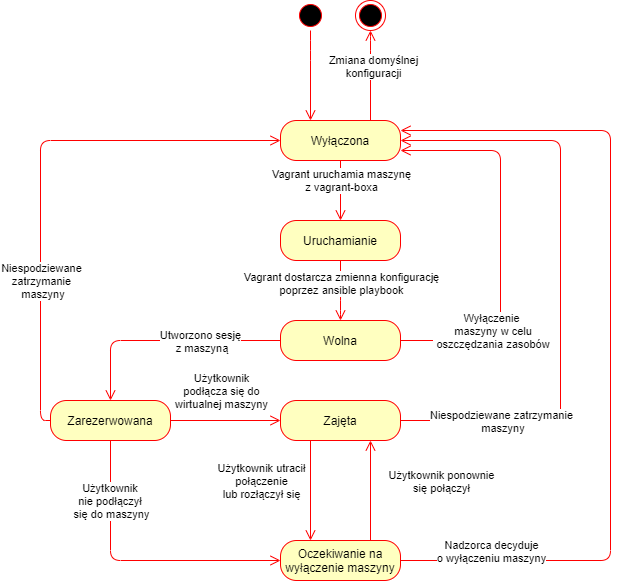
\includegraphics[width=\textwidth]{state_diagrams/virtual_machine.png}
	
	\vskip-1.5ex
	
	\caption{Diagram stanów dla maszyny wirtualnej}
	\label{state_vm}
\end{figure}

Maszyna aby być całkowicie uruchomiona musi być zaopatrzona we wszystkie konfiguracje.
Stan "Wolna" oznacza możliwość przypisania sesji do tej maszyny w razie potrzeby.
Po rezerwacji użytkownik nie musi od razu się zalogować (posiada pewien czas na podłączenie się do systemu).
Maszyna przy oczekiwaniu na podłączenie się użytkownika (również po zerwaniu połączenia) oczekuje w stanie "Oczekiwanie na wyłączenie maszyny".
Gdy użytkownik pracuje na maszynie (wiemy o tym przez monitorowanie kolejki zdefiniowanej w \hyperref[external-modules:broker:queue-users]{opisie kolejki użytkowników}) wtedy jest ona w stanie "Zajęta".
\pagebreak

\subsubsection{Serwer wirtualizacji}

Serwer wirtualizacji monitoruje zasoby zużywane przez uruchamiane no nim wirtualne maszyny oraz fakt podłączenia do niego użytkowników.

\begin{figure}[!h]
	
	\centering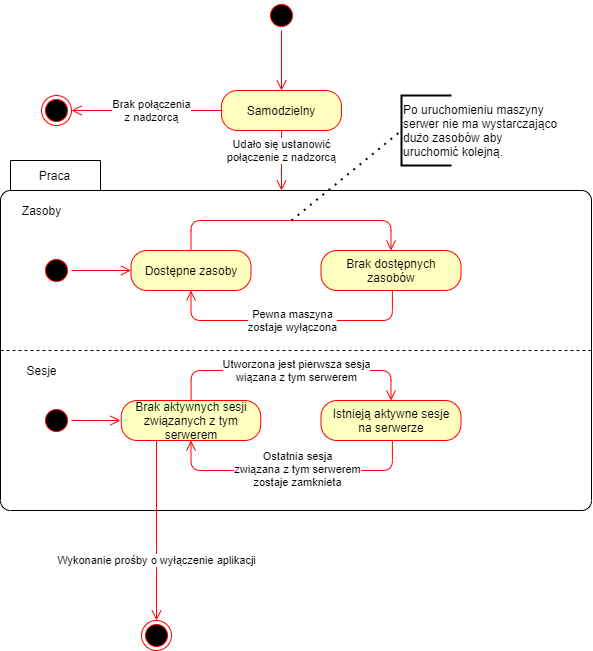
\includegraphics[width=0.8\textwidth]{state_diagrams/virtualisation_server.png}
	
	\vskip-1.5ex
	
	\caption{Diagram stanów dla serwera wirtualizacji}
	\label{state_virtsrv}
\end{figure}

Przy starcie serwer wirtualizacji oczekuje działającego nadzorcy w sieci.
Jeżeli się taki nie znajdzie kończy się z błędem.
Gdy jednak odnajdzie takowy rozpoczyna się praca serwera.
Ze względu na zasoby może on mieć wolne zasoby aby utworzyć nowe maszyny, lub też nie.
Jednak ważniejszym stanem z perspektywy działania serwera są podłączeni do niego użytkownicy.
W przypadku gdy podłączony jest do niego przynajmniej jeden użytkownik nie może się zakończyć jego praca.
Jeżeli system ma wyłączyć się prawidłowo ostatni użytkownik musi rozłączyć się z używana maszyną wirtualną.
\pagebreak

\subsubsection{Użytkownik}

\begin{figure}[!h]
	
	\centering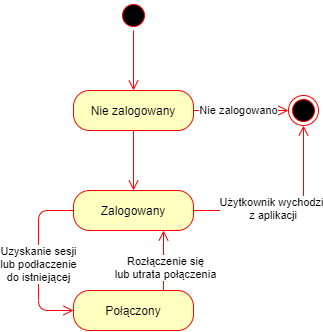
\includegraphics[width=\screenswidthlesser]{state_diagrams/client.png}
	
	\vskip-1.5ex
	
	\caption{Diagram stanów dla użytkownika}
	\label{state_user}
\end{figure}

Użytkownik z perspektywy systemu po zalogowaniu może być 2 dwóch stanach: pracuje w ramach swojej sesji lub też nie.
W stanie "Połączony" aplikacja na której pracuje ma obowiązek powiadamiać serwer wirtualizacji, że ciągle jest obecny.
Przy zmianie stanu do innego informowanie musi ustać.


\end{document}